% Preamble: \usepackage{graphicx}; set \graphicspath to ../figures/ as appropriate.
\begin{figure*}[t]
  \centering
  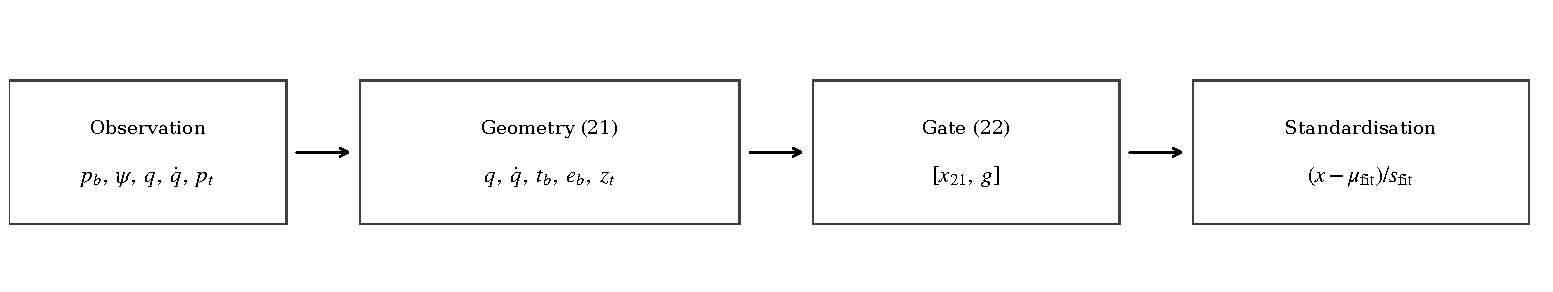
\includegraphics[width=\textwidth]{feature_pipeline.pdf}
  \caption{Feature construction for teacher A. The 21-dimensional base
    representation contains joint state, robot-relative target geometry,
    FK target error and world target height. The gate variant appends one
    observable reach-active indicator before fitting-only standardisation.}
  \label{fig:feature-pipeline}
\end{figure*}

\begin{figure*}[t]
  \centering
  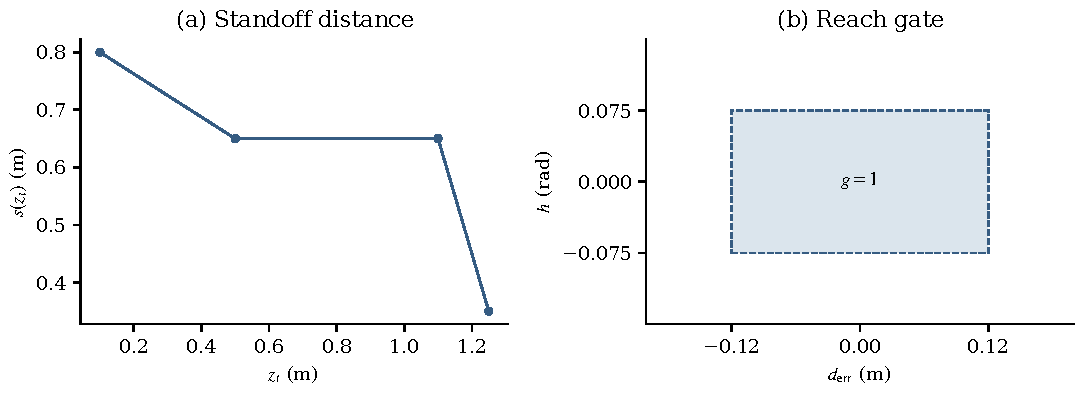
\includegraphics[width=\textwidth]{reach_gate.pdf}
  \caption{(a) Height-dependent standoff distance. (b) Reach gate in distance
    error and heading error: $g=1$ only where $|d_{\mathrm{err}}|<0.12$\,m
    and $|h|<0.075$\,rad. The dashed boundary is excluded. The gate is
    reconstructed from current deployable features, without teacher memory.}
  \label{fig:reach-gate}
\end{figure*}

\begin{figure*}[t]
  \centering
  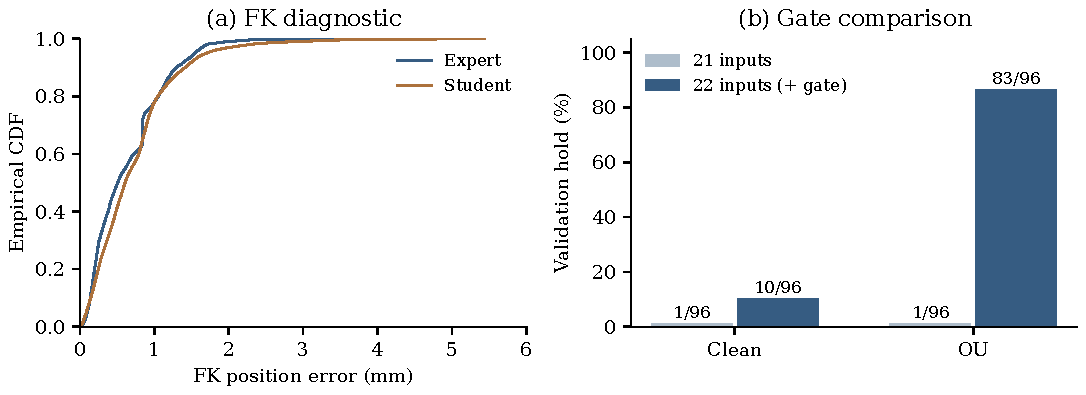
\includegraphics[width=\textwidth]{feature_evidence.pdf}
  \caption{(a) Deployed FK error on four nominal fitting scenarios per role,
    sampled every 10\,ms. The student is the archived 27 October DAgger
    round-1 student, not ablation row R1. (b) Gate comparison for the fixed
    v1 rows R1--R4, pooled over three training seeds on the same 32 validation
    scenes. Each denominator is 96 rollouts, not 96 distinct scenarios.}
  \label{fig:feature-evidence}
\end{figure*}
